\documentclass[conference]{IEEEtran}
\usepackage{cite}
\usepackage{amsmath,amssymb,amsfonts}
\usepackage[brazilian]{babel}
\usepackage{algorithmic}
\usepackage{graphicx}
\usepackage{textcomp}
\usepackage{xcolor}
\usepackage{verbatim}
\usepackage{hyperref}
\usepackage{url}
\usepackage{physics, mathtools}
\usepackage{tabularx, scalefnt}
\usepackage{multicol, multirow}
\usepackage{pdfpages}
\IEEEoverridecommandlockouts

\IEEEoverridecommandlockouts 


\title{\LARGE \bf Controlador PID para regular o nível de água na bancada de controle de processos industriais}
\author{Henrique Fragoso, \textit{Engenharia de Controle e Automação}, IFC $^{1}$ 
\\ João Guilherme Carvalho, \textit{Engenharia de Controle e Automação}, IFC $^{2}$
\\ Marcelo Ancelmo, \textit{Engenharia de Controle e Automação}, IFC $^{3}$
\\ Naime Aiub, \textit{Engenharia de Controle e Automação}, IFC $^{4}$
\thanks{$^{1}$Fragoso, H. {\tt\small heriquebati@gmail.com}, $^{2}$Carvalho, J.G. {\tt\small joãogcarvalho012@gmail.com}, $^{3}$Ancelmo, M. {\tt\small marceloancelmomx2@gmail.com} $^{4}$Aiub, N. {\tt\small naimeaiub@gmail.com}}
}



\date{}
\begin{document}
\maketitle
\thispagestyle{plain}
\pagestyle{empty}



\begin{abstract}
    Quando os modelos matemáticos da planta são desconhecidos, faz-se necessário a utilização de métodos heurísticos, 
    que se baseia em obter os parâmetros necessários à partir de ensaios realizados e gráficos com curva padrão. 
    Esses métodos foram assunto de estudos de diversas frentes, entre elas as mais famosas Ziegler-Nichols (Z\&N) e CHR,
     sendo essas utilizadas no trabalho. O objetivo do seguinte documento, é realizar testes na bancada de controle 
     de nível e utilizar dos métodos citados para realização do controle PID, de forma a comparar os resultados obtidos 
     dos diferentes métodos. Isso porque se adéquam melhor dependendo das características do sistema, 
     esse que por sua vez foi a bacada disposta pelo IFC \textit{campus} São Bento do Sul. 
     Dos resultados obtidos e comparações realizadas, temos dois sistemas que obtiveram êxito, 
     sendo necessário alguns ajustes de ganho. Porém, diferem entre a velocidade de resposta e sobressinal aceitável, 
     uma sintonia do controlador PID mais rápida (Z\&N) e outra mais lenta, mas sem overshoot (CHR), findando assim o 
     documento com êxito.

    Palavras-chave\textit{ - }CHR, Controle PID, Métodos heurísticos, Ziegler-Nichols.
\end{abstract}

\section{Introdução}

São imensas as vantagens que a adição de um controlador pode trazer ao processo industrial na qual é inserido, como a rapidez, a otimização, a estabilidade, e entre vários outras especificações do desempenho, e os parâmetros do controlador estão diretamente relacionados a isso. Através da bancada de controle de processos, é possível executar processos comuns a indústria, como o controle de nível, temperatura, pressão, ou de vazão. Na bancada pode ser utilizado controle do tipo Proporcional-Integral-Derivativo (PID).

O foco do estudo do artigo está no projeto de um controlador do tipo PID, utilizando os métodos heurísticos de sintonia  para controlar a alteração de nível da bancada de controle. Os métodos utilizados para parametrizar os valores do controlador se baseiam em valores retirados da curva de reação do sistema a uma resposta em degrau. A resposta do sistema deve ser como um 'S' e dessa resposta são retiradas valores para os cálculos dos parâmetros do controlador. Os cálculos são tabelados, e cada método tem sua a sua tabela.

Os objetivos do projeto são os testes do controle na bancada de processos e uma comparação entre dois métodos heurísticos em relação a resposta sem controlador, sendo o segundo método de Ziegler-Nichols e CHR com resposta mais rápida sem sobressinal. O software de supervisão utilizado foi o \textit{Elipse SCADA}.

\section{Fundamentação Teórica}

\subsection{Bancada Didática de Controle de Processos Industriais}

O objeto de estudo de controle do artigo é a bancada de controle de processos industriais (Figura \ref{figura:bancada}), com foco no processo de nível presente na bancada. A bancada possui vários mecanismos  para o controle dos processos como, por exemplo, sensores e controladores, o que propicia uma vivência na industria.

A bancada didática a ser trabalhada é constituída de sensores que capturam estímulos físicos na planta e fornecem dados correspondentes;  controlador lógico programável (CLP) que recebe esses dados e enviam sinais de controle aos atuadores , que executam comandos de outros dispositivos, como um motor ligando. Na parte de software, sistemas de controle agem sobre os controladores para que executem funções especificadas e sistemas de supervisão permitem a coleta de dados do sistema, e também a interação do operador com sistema através de telas de comando \cite{auttom}.

\begin{figure}[!http]
    \centering
    \caption{Bancada de controle de processos industriais}
    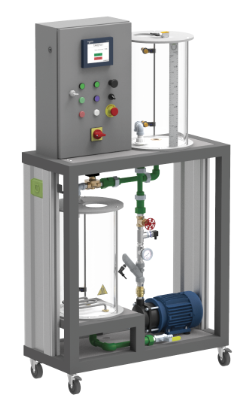
\includegraphics[width=0.2\textwidth]{imagens/Bancada.png}\\
    Fonte: \cite{auttom}
    \label{figura:bancada}
\end{figure}

\subsection{Ziegler-Nichols}

Quando o modelo matemático da planta não é conhecido e os métodos de projeto analíticos não podem ser utilizados, são empregados os métodos heurísticos de controle PID. Onde conferem grande aplicabilidade em diversas situações, como por exemplo na indústria, obtendo resultados satisfatórios, mas podendo não ser excelentes.

Ziegler-Nichols (Z\&N) propuseram dois métodos, em 1942, para obter as funções de controle de modo heurístico. Os dois métodos básicos visam obter mesma resposta especificada para o sistema em malha fechada, e diferem no que diz respeito à natureza da informação sobre a dinâmica do processo que é exigida por cada um deles \cite{teixeira2010controles}.

Ambos se baseiam na dinâmica SISO (“\textit{Single Input Single Output”}). Onde há regras para a sintonia dos controladores PID (ajuste dos valores de \(K_{p}\), \(T_{i}\) e \(T_{d}\))  fundamentado na resposta experimental ao degrau ou no valor de \(K_{p}\) \cite{teixeira2010controles}.

Sintonizar um controlador se refere a selecionar parâmetros do controlador para garantir determinada especificação \cite{ogata2011engenharia}.

O modelamento matemático por função de transferência (FT) que representa as ações derivativa e integrativa é dado em uma relação entre U(s) que representa ação de controle (a maneira que o controlador automático produz o sinal de controle), e E(s) que é o erro do sinal de saída em relação a entrada que serve de referência \cite{ogata2011engenharia}:

\begin{equation}
    \frac{U(s)}{E(s)} = K_p   (1 + \frac{1}{T_I S} + T_D S)
\end{equation}

\subsection{Segundo método de Ziegler-Nichols}

No segundo método é obtido experimentalmente a resposta da planta a uma entrada degrau unitário, não havendo integradores ou polos complexos conjugados dominantes, a curva de resposta será como 'S', onde é caracterizada por duas constantes (Figura \ref{figura:degrau}), atraso (L = \(\theta\)) e a constante de tempo (T = \(\tau\)) \cite{teixeira2010controles}.

\begin{figure}[!http]
    \centering
    \caption{Resposta da planta ao degrau unitário.}
    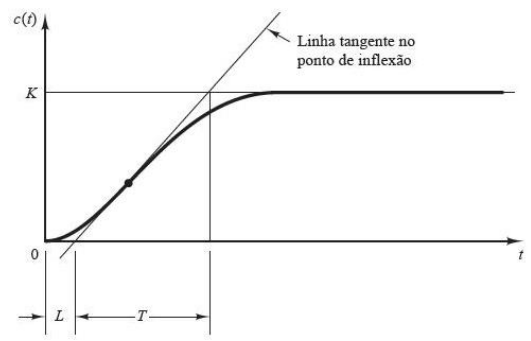
\includegraphics[width=0.35\textwidth]{imagens/degrau_Z&N.png}\\
    Fonte: \cite{teixeira2010controles}
    \label{figura:degrau}
\end{figure}

Para a determinação da sintonia do controlador PID, são necessários os valores de \(\theta\), \(\tau\) e K. Onde \(\tau\) e \(\theta\) vem da curva de resposta ao degrau, enquanto que para o K (ganho do processo) utiliza \(\Delta u\) e \(\Delta y\) (Figura \ref{figura:constantes}), que são normalizados pelo range do instrumento de medição utilizado no processo \cite{teixeira2010controles}.

\begin{figure}[!http]
    \centering
    \caption{Parâmetros obtidos pela resposta da planta ao degrau unitário.}
    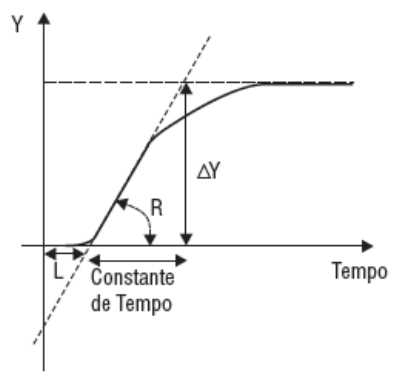
\includegraphics[width=0.35\textwidth]{imagens/constantes_Z&N.png}\\
    Fonte: \cite{teixeira2010controles}
    \label{figura:constantes}
\end{figure}

Onde,
\begin{equation}
    \Delta y  (100\%) = \frac{\Delta y}{range} * 100
    \label{deltay}
\end{equation}
\begin{equation}
    K = \frac{\Delta y (100\%)}{\Delta u (100\%)}
    \label{K}
\end{equation}
\newpage
Com os valores de \(\tau\), \(\theta\) e K, podemos definir a sintonia a partir da tabela \ref{sintonia}.

\begin{table}[!h]
    \centering
    \caption{Sintonia do controlador pelo segundo método de Z\&N}
    \begin{tabular}{|c|c|c|c|} \hline
        Controlador & \(K_p\)                          & \(T_i\)           & \(T_D\)          \\ \hline
        P           & \(\tau\) / (K x \(\theta\))      & -                 & -                \\ \hline
        PI          & 0.9  \(\tau\) / (K x \(\theta\)) & 3.33 x \(\theta\) & -                \\ \hline
        PID         & 1.2  \(\tau\) / (K x \(\theta\)) & 2 x \(\theta\)    & 0.5 x \(\theta\) \\ \hline
    \end{tabular}\\
    \label{calczn}
    Fonte: \cite{teixeira2010controles}.
    \label{sintonia}
\end{table}

\subsection{CHR - Resposta mais rápida sem sobressinal}

O método de Chien, Hrones e Reswick (CHR) propõe dois critérios de desempenho: uma seria a resposta mais rápida sem sobressinal; e a outra a resposta mais rápida com com 20\% de sobressinal \cite{teixeira2010controles}. Foi optado pelo primeiro critério, porque dificilmente uma resposta rápida é necessário para grande parte dos processos industriais, além disso, por escolher um sistema mais lento, o ganho do mesmo é menor, deixando o sistema menos propício a instabilidade \cite{teixeira2010controles}. A tabela \ref{sintoniaCHR} mostra as fórmulas para chegar a sintonia do controlador PID pelo método CHR para o critério em questão.

\begin{table}[!h]
    \centering
    \caption{Sintonia do controlador pelo método CHR}
    \begin{tabular}{|c|c|c|c|} \hline
        Controlador & \(K_p\)                              & \(T_i\)         & \(T_D\)          \\ \hline
        P           & (0.3 x \(\tau\)) / (K x \(\theta\))  & -               & -                \\ \hline
        PI          & (0.35 x \(\tau\)) / (K x \(\theta\)) & 1.16 x \(\tau\) & -                \\ \hline
        PID         & (0.6 x \(\tau\)) / (K x \(\theta\))  & \(\tau\)        & 0.5 x \(\theta\) \\ \hline
    \end{tabular}\\
    \label{calcchr}
    Fonte: \cite{teixeira2010controles}.
    \label{sintoniaCHR}
\end{table}


\section{Metodologia}

\subsection{Aquisição de dados}

Inicialmente, foi necessário realizar uma comunicação entre o software de supervisão e aquisição de dados (\textit{Elipse SCADA}), o CLP da bancada, e o software \textit{TIA PORTAL V15}, - qual é necessário para obter a programação contida no CLP e os endereços de memória dos dados que seriam supervisionados através do software \textit{SCADA}. Após esta conexão feita, foi executado testes no sistema em malha aberta a partir de uma entrada em degrau.

Para a execução destes testes era necessário ligar manualmente tanto a bomba quanto a válvula e definir uma frequência inicial para o motor da bomba. Após o sistema ficar estável nesta frequência, o mesmo foi excitado a uma entrada em degrau, ou seja, alterou-se a frequência inicial. Através do \textit{Elipse SCADA} foi possível estabelecer um monitoramento da bancada possibilitando a extração de dados relativos aos pontos de níveis em relação ao tempo, para realizar o projeto de um controlador PID para o nível de água no reservatório. A figura \ref{figura:dados} apresenta o gráfico gerado no \textit{Excel} a partir dos valores retirados do software de supervisão e o momento em que foi aplicado um degrau na entrada.

\begin{figure}[!http]
    \centering
    \caption{Resposta adquirida através do software \textit{Elipse SCADA}}
    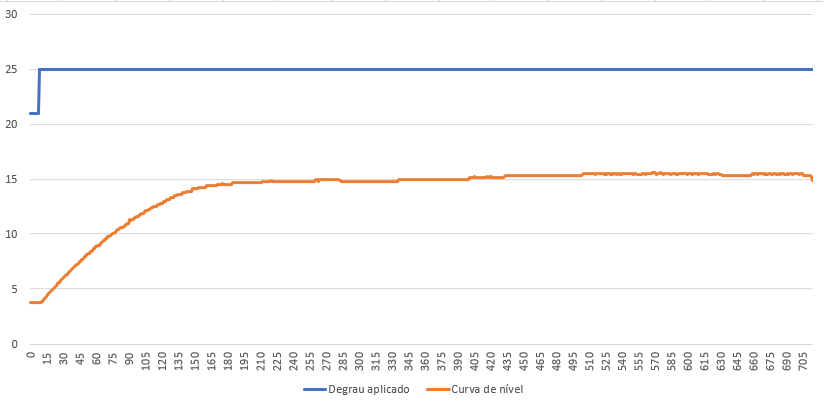
\includegraphics[width=0.4\textwidth]{imagens/dadosextraido.png}\\
    Fonte: O autor.
    \label{figura:dados}
\end{figure}

\subsection{Projeto do controle PID}
Em posse do gráfico da figura \ref{figura:dados}, e das equações \ref{deltay} e \ref{K}, foi determinado os parâmetros $\theta$, $\tau$, $K$. Tais parâmetros são utilizados nos métodos de sintonia de Z\&N e CHR para encontrar os valores de $K_p$, $T_i$ e $T_d$, os quais são calculado através das equações das tabelas \ref{sintonia} e \ref{sintoniaCHR}.


Como na prática o sistema não tem configurações ideais, como as calculadas, se é necessário ajustar o ganho manualmente para evitar instabilidades. O ganho $K_p$ então deveria ser diminuído e depois aumentado de forma gradativa enquanto se realizara testes. Porém, a bancada utilizada mostrou-se um problema no qual o ganho $K_p$ apresentava uma resposta invertida ao seu funcionamento normal. Normalmente um ganho $K_p$ pequeno apresenta menor velocidade de ação, e um $K_p$ maior apresenta maior velocidade de ação e também maiores oscilações. Por este motivo, para o ajuste manual de $K_p$, seu valor foi inicialmente aumentado e em seguida diminuído conforme alguns testes.


\section{Resultados}

\subsection{Parâmetros $\theta$, $\tau$, $K$}
Através da análise realizada no gráfico da figura \ref{figura:dados} e da equação \ref{K} foi determinado os parâmetros $\theta$, $\tau$, $K$, sendo eles 1.5, 90 e 10.28, respectivamente. Para validação dos dados retirados da curva 'S', é possível realizar uma aproximação a uma função de transferência de primeira ordem (equação \ref{aproximacao}).

\begin{equation}
    G(s) = \frac{Ke^{-\theta s}}{\tau s + 1} = \frac{10.28e^{-1.5 s}}{90s + 1}
    \label{aproximacao}
\end{equation}

Na seguinte figura, esta aproximação pode ser vista ao comparar o gráfico adquirido através do software \textit{Matlab} da função de transferência aproximada e da curva 'S' extraída da bancada. Visto que é uma aproximação e os parâmetros são extraídos manualmente do gráfico, as respostas não irão se sobrepor, mas serão semelhantes. Para a comparação, se foi realizado um \textit{offset} no gráfico adquirido, deixando seu ponto inicial em 0.

\begin{figure}[!http]
    \centering
    \caption{Comparação entre a FT e a resposta adquirida}
    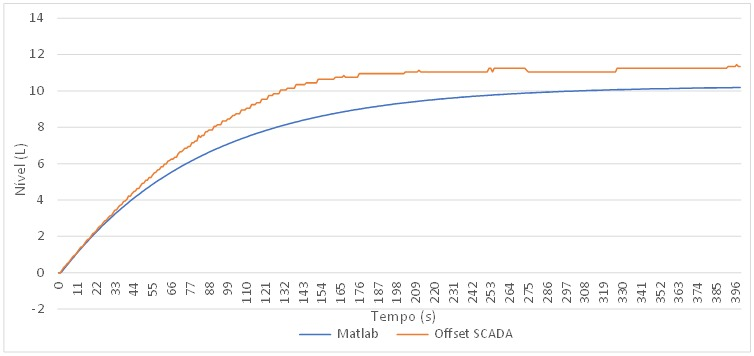
\includegraphics[width=0.45\textwidth]{imagens/Aproximacao.jpeg}\\
    Fonte: O autor.
    \label{figura:aprox}
\end{figure}

\subsection{Parâmetros \(K_p\), \(T_i\), \(T_d\)}

A partir dos parâmetros encontrados e das tabelas \ref{calczn} e \ref{calcchr}, foi calculado os valores de $K_p$, $T_i$, $T_d$ para o controle PID pelo método Z\&N e CHR, como segue a tabela seguinte.
\begin{table}[!h]
    \centering
    \caption{Parâmetros \(K_p\), \(T_i\) e \(T_d\) }
    \begin{tabular}{|c|c|c|c|} \hline
        $Sintonia$ & $K_p$ & $T_i$ & $T_d$  \\ \hline
        $Z\&N$     & 7   & 3   & 0.75 \\ \hline
        CHR      & 3.5 & 90  & 0.75 \\ \hline\end{tabular}
\end{table}\\
Com estes valores, é possível obter a função dos compensadores em ambos métodos utilizando a equação \ref{funcaocomp}.
\begin{equation}
    G_c(s) = K_p(1+ \frac{1}{sT_i}+sT_d)
    \label{funcaocomp}
\end{equation}

\subsection{Análise dos resultados}

Como dito anteriormente, foi-se realizado alguns testes com o valor de $K_p$ maior, e logo após sendo diminuído. Para critérios de análise, foi-se escolhido a resposta de cada método utilizando dois ganhos diferentes, um alto e o outro calculado (O método CHR não foi utilizado o ganho calculado pois quando utilizando o mesmo, a bancada não chegava a iniciar seu processo).

Podemos observar através da figura \ref{CHR}, que quando utilizado o método CHR no qual não apresenta \textit{overshoot}, o sistema possui uma resposta demasiada lenta. Pode-se ver também que utilizando um ganho menor, o sistema é mais rápido, entretanto essa informação não é muito visível já que, por possuir um tempo morto muito elevado, o sistema com ganho maior chega ao nível desejado primeiro.

\begin{figure}[!http]
    \centering
    \caption{Comparação do método CHR com diferentes ganhosR}
    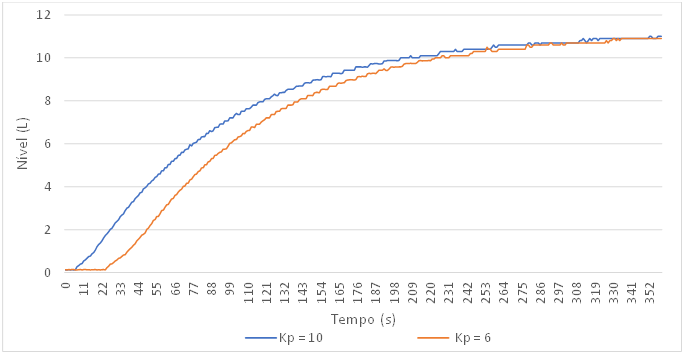
\includegraphics[width=0.45\textwidth]{imagens/grafico_CHR.png}\\
    Fonte: O autor.
    \label{CHR}
\end{figure}

Quando utilizado o método Z\&N, a resposta é mais rápida, contendo um grande \textit{overshoot}, o que implica em uma grande máximo sobressinal e um tempo de acomodação maior, ao se utilizar o ganho \(K_p\) calculado. E aumentando o ganho, faz com que o \textit{overshot} e o tempo de acomodação seja menor.

\begin{figure}[!http]
    \centering
    \caption{Comparação do método Z\&N com diferentes ganhos}
    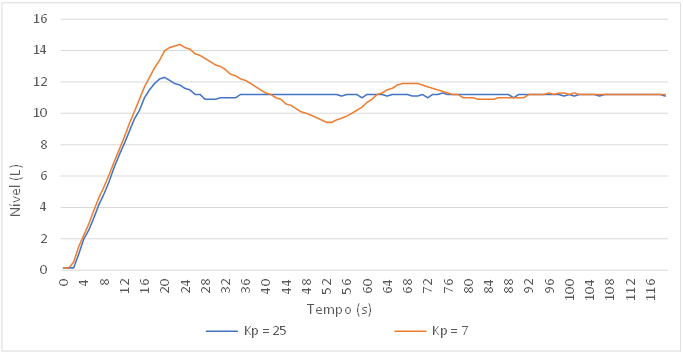
\includegraphics[width=0.5\textwidth]{imagens/grafico_Z&N.png}\\
    Fonte: O autor.
    \label{ZN}
\end{figure}

E por fim, foi comparado a resposta dos dois métodos utilizados Nota-se pela figura \ref{ZNCHR}, que quando utilizado o método Z\&N a resposta obtida é mais rápida e com um pequeno \textit{overshot} de aproximado 10\%. Logo, caso seja necessário uma resposta rápida e que aceite um pequeno máximo sobressinal, o método de Ziegler-Nichols será bem utilizado. Porém, se a resposta não pode haver um \textit{overshot}, o método CHR se sobressai e será o mais adequado.

\begin{figure}[!http]
    \centering
    \caption{Comparação entre o método Z\&N e CHR}
    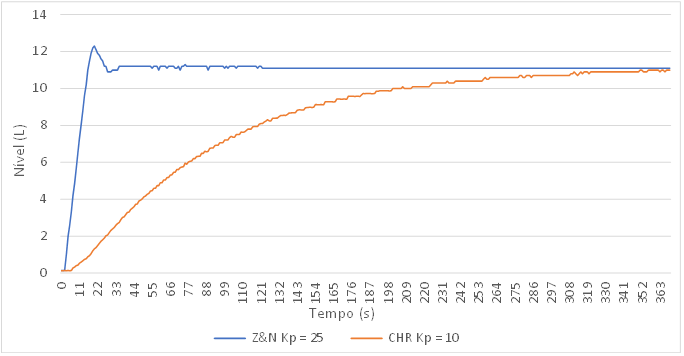
\includegraphics[width=0.5\textwidth]{imagens/grafico_Z&N_CHR.png}\\
    Fonte: O autor.
    \label{ZNCHR}
\end{figure}

\section{Conclusão}
Apesar das dificuldades em realizar a comunicação entre o software \textit{Elipse SCADA} e o CLP; e a bancada não responder de forma esperada a alteração do ganho $K_p$, o projeto do controle PID para a bancada de processos industriais apresentou um funcionamento de forma satisfatória. Dependendo da aplicação do projeto, há a necessidade de uma resposta mais rápida ou mais lenta. Com a comparação dos dois métodos utilizados neste trabalho, é possível observar que aplicando o método Z\&N é obtido uma resposta mais rápida do que a resposta do sistema com o controlador PID que utiliza-se o método CHR. Cabe ao projetista definir o método de melhor aplicação.

As teorias baseadas para definições de parâmetros e os dados obtidos através dos softwares foram satisfatório. Com isso, tem-se que o projeto proposto e os objetivos estabelecidos foram cumpridos, dado que foi possível realizar dois projetos de controle PID e implementa-los na bancada de controle.


\addtolength{\textheight}{-12cm}
\bibliographystyle{IEEEtran}
\bibliography{references}

\end{document}